\documentclass[conference,letterpaper]{IEEEtran}
\usepackage{mathptmx}
\usepackage[T1]{fontenc}
\usepackage{graphicx,amsmath,booktabs,url,tikz}
\usetikzlibrary{arrows.meta,positioning}
\title{Chip Orchestra for Observable RTL to Padframe Design}
\author{\IEEEauthorblockN{Ade Irman Budi Hendrawan, William Anthony, Rifky Afriadi, Radhian Ferel Armansyah}
\IEEEauthorblockA{School of Electrical Engineering and Informatics\\Bandung Institute of Technology (ITB)\\Bandung, Indonesia\\
\{adeirman2705, willomooi, rifki.afriyadi, radhianarmansyah\}@gmail.com}}
\begin{document}
\maketitle
\begin{abstract}
Open-source implementation tools provide access to digital chip design, but translating generated hardware into a chip-level padframe requires coordinated behavioral checks, physical artifacts, and acceptance decisions. We present Chip Orchestra, an observable orchestration platform that connects executable reference models, hierarchical register-transfer-level generation, electronic design automation tools, and GlobalFoundries 180 nm padframe assembly. The platform preserves stage reports and raw tool logs, supports bounded repair, and exposes reference outputs for human approval before hardware generation. We evaluate its implementation backend with a serially connected NanoCGRA array containing nine processing elements and 32 bytes of memory. Fresh simulation passes four end-to-end functional transactions, and fresh synthesis produces 129,736.32 square micrometers of mapped cell area. A separate assembly run integrates the retained 466.555 micrometer square physical core into a 2.935 mm square ring, producing a binary chip-level layout with 993 cell definitions, four signal routes, and seven supply routes. Independent KLayout readback confirms the ring and translated core hierarchy, and the resulting layout is shown directly. The fresh hardening attempt stops before placement because of a timing-tool compatibility error. Pad-to-core routes remain geometric, with electrical connectivity and full-chip physical verification pending. The work demonstrates reproducible backend execution and an inspectable core-to-padframe handoff while making the boundary between assembly and fabrication readiness explicit.
\end{abstract}
\begin{IEEEkeywords}
RTL to padframe, chip design automation, hardware verification, open-source EDA, AI orchestration
\end{IEEEkeywords}

\section{Introduction}
Generating register-transfer-level (RTL) code does not complete an application-specific integrated circuit (ASIC). The circuit must satisfy its behavioral specification, map to a technology library, meet implementation constraints, and connect to external signals and supplies through an input/output (I/O) padframe. Errors can arise at the transitions between these tasks even when individual tools finish successfully. An execution system must therefore preserve both the artifacts produced and the scope of the checks applied to them.

OpenROAD provides an open-source foundation for digital physical implementation~\cite{openroad}, while LibreLane coordinates synthesis, implementation, and verification steps~\cite{librelane}. These tools enable a reproducible core-design flow, but projects still need to connect behavioral intent, generated RTL, engineering review, and chip-level integration. Large language models (LLMs) make this coordination especially relevant because generated code and revised constraints must be evaluated against explicit acceptance criteria.

Chip Orchestra addresses this problem through observable task stages. Its contribution combines three interfaces. An executable reference-model gate exposes the interpreted behavior before RTL generation. Structured stage reports associate artifacts and diagnostics with execution attempts and bounded repair. A padframe backend places a hardened core inside a reusable GlobalFoundries 180 nm microcontroller (GF180MCU) ring and exports a chip-level layout. The contribution is this coordinated handoff, rather than a new placement or routing algorithm.

We evaluate the backend using NanoCGRA, a coarse-grained reconfigurable array (CGRA) whose four-signal serial interface matches the available ring configuration. The evaluation distinguishes fresh simulation and synthesis from a newly executed assembly that reuses an existing physical core. This distinction makes failures and completed results inspectable without attributing old implementation metrics to a new run. The central question is what evidence the orchestration retains as a design crosses from functional RTL to core implementation and padframe assembly.

Section II describes the platform and assembly method. Section III presents the NanoCGRA setup and reproduction procedure. Section IV reports the functional, synthesis, and layout results. Section V discusses their scope and limitations. Section VI concludes the paper.

\section{Platform and Assembly Method}
\subsection{Observable Execution}
The platform separates a browser interface, a Go orchestration service, a Python agent service, and a Python electronic design automation (EDA) service. MySQL stores task state and Redis supports event delivery. A directed acyclic graph represents stage dependencies. Reports contain metrics, artifact paths, summaries, warnings, errors, and raw log locations. Fig.~\ref{fig:flow} shows the logical workflow. It describes platform capabilities, not stages demonstrated by the present backend experiment.

The golden-reference stage generates executable Python behavior, test suites, and input/expected-output vectors. Successful generation enters an awaiting-approval state. The engineer reviews the reference output before RTL generation is released. This gate exposes a specification interpretation that compilation alone cannot validate. Generated RTL is organized into leaf modules, intermediate integrators, and a chip top, with self-checking testbenches for behavioral comparison.

Repair loops consume diagnostics under a configured budget. Verification must apply to the resulting files after a repair, because earlier results describe a different candidate. Physical metrics must also retain their clock, corner, and implementation stage. A successful behavioral test at a chosen simulation clock is not evidence that the physical implementation meets that frequency.

\begin{figure}[t]
\centering
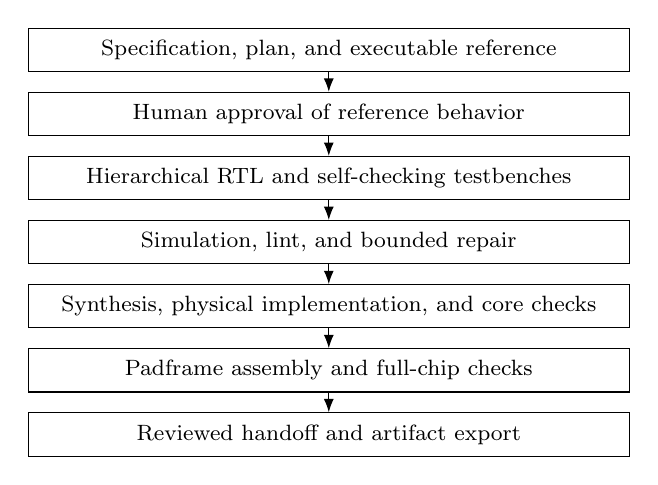
\begin{tikzpicture}[node distance=2.5mm,box/.style={draw,align=center,text width=7.4cm,minimum height=5.5mm,font=\footnotesize},>=Latex]
\node[box] (a) {Specification, plan, and executable reference};
\node[box,below=of a] (b) {Human approval of reference behavior};
\node[box,below=of b] (c) {Hierarchical RTL and self-checking testbenches};
\node[box,below=of c] (d) {Simulation, lint, and bounded repair};
\node[box,below=of d] (e) {Synthesis, physical implementation, and core checks};
\node[box,below=of e] (f) {Padframe assembly and full-chip checks};
\node[box,below=of f] (g) {Reviewed handoff and artifact export};
\foreach \s/\t in {a/b,b/c,c/d,d/e,e/f,f/g}{\draw[->] (\s)--(\t);}
\end{tikzpicture}
\caption{Logical platform workflow. The evaluation invokes EDA backend runners directly and does not exercise LLM generation or the reference-approval gate.}
\label{fig:flow}
\end{figure}

\subsection{Core and Padframe Artifacts}
The EDA service invokes Icarus Verilog for simulation and syntax checking, Verilator for static analysis, Yosys for synthesis, and LibreLane/OpenROAD for physical implementation. GF180MCU supplies the process design kit (PDK), standard-cell views, I/O cells, and physical rules~\cite{gf180}. The service retains structured reports even when a tool fails, so an unsuccessful physical stage can be distinguished from successful functional or synthesis stages.

The \texttt{gf180-v1} padframe configuration specifies a $2935\times2935\,\mu$m die and a $0.005\,\mu$m grid. It declares 58 analog pads, two digital inputs for clock and reset, two bidirectional pads for a universal asynchronous receiver/transmitter (UART), three digital supply pads, four digital ground pads, and four corners. These are reusable ring resources. The application uses four signal pads, rather than exercising all 69 configured I/O resources.

The native Python assembler reads the ring and core Graphic Data System II (GDSII) files using \texttt{gdspy}. It rejects missing input files, missing top-level cells, and unavailable bounding boxes. It merges cell libraries, prefixes colliding core cell names, creates a chip top, and inserts ring and core references. For ring and core bounding-box centers $\mathbf{c}_r$ and $\mathbf{c}_c$, respectively, the translation is
\begin{equation}
\mathbf{t}=\mathbf{c}_r-\mathbf{c}_c .
\label{eq:translation}
\end{equation}
Here $\mathbf{t}$ is the two-dimensional core offset. The assembled hierarchy preserves the reusable ring and core beneath a common chip top. Containment and keep-out requirements must be checked against the usable ring opening, not only its outer bounding box.

\subsection{Routing and Handoff Scope}
Clock and reset use south-edge input pads, while UART signals use west-edge bidirectional pads. Signal names are matched against core pins from the Design Exchange Format (DEF) file. The backend draws signal routes on Metal2 and supply straps on Metal3. However, endpoints are calculated from approximate pad geometry and distributed core-edge positions, rather than extracted pin shapes. The current implementation therefore generates geometric connections, whose electrical validity requires separate verification.

The backend emits binary GDSII, a resolved pad configuration, supporting DEF, a Library Exchange Format (LEF) abstract, a ring netlist, previews, and a log. If the historical external padring binary is unavailable, deterministic supporting files are produced. Native GDSII assembly remains the primary path. Neither file creation nor the report's binary-generation indicator establishes design-rule checking (DRC) or layout-versus-schematic (LVS) acceptance.

\section{Experimental Setup}
\subsection{NanoCGRA Workload}
NanoCGRA-Lite contains a $3\times3$ mesh of nine processing elements, 32 bytes of static random-access memory (SRAM), a controller, and a UART bridge. Its top-level signals are \texttt{clk}, \texttt{rst\_n}, \texttt{uart\_rx}, and \texttt{uart\_tx}. Fig.~\ref{fig:nano} shows the application-level data path. The bridge decodes a three-byte command packet containing command, address, and data. Write, read, and run commands access the internal eight-bit memory-mapped interface.

\begin{figure}[t]
\centering
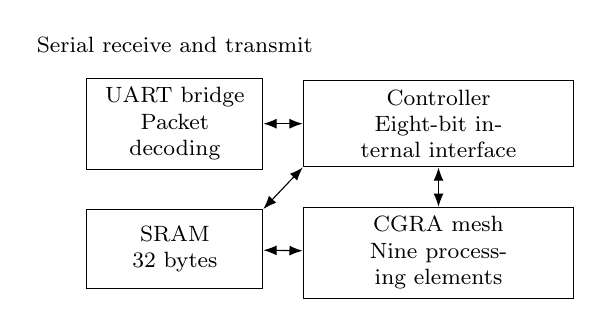
\begin{tikzpicture}[node distance=5mm,box/.style={draw,align=center,font=\footnotesize,minimum height=10mm},>=Latex]
\node[box,text width=2cm] (uart) {UART bridge\\Packet decoding};
\node[box,text width=3.2cm,right=of uart] (ctrl) {Controller\\Eight-bit internal interface};
\node[box,text width=2cm,below=of uart] (sram) {SRAM\\32 bytes};
\node[box,text width=3.2cm,below=of ctrl] (array) {CGRA mesh\\Nine processing elements};
\draw[<->] (uart)--(ctrl);
\draw[<->] (ctrl)--(array);
\draw[<->] (ctrl.south west)--(sram.north east);
\draw[<->] (sram)--(array);
\node[font=\footnotesize,above=2mm of uart] {Serial receive and transmit};
\end{tikzpicture}
\caption{NanoCGRA application-level organization. The UART interface provides the four-signal boundary used by the padframe configuration. Clock and reset are shared.}
\label{fig:nano}
\end{figure}

The integration testbench writes operands and configuration, initiates computation, reads the result through UART, and checks the expected value. It covers SRAM readback, addition, multiplication, and exclusive-or. The test clock has a 100 ns period, with eight clocks per UART bit in the testbench override. Assertions exercise the complete transaction through the RTL interface, rather than only a processing-element unit.

\subsection{Execution and Provenance}
The experiment uses repository revision \texttt{4f20f65}. RTL and testbenches are copied from the optimized NanoCGRA workspace into a separate run directory. The top-level testbench's verdict strings are adapted to the runner's expected \texttt{TEST PASSED} and \texttt{TEST FAILED} format, and a top-level waveform dump is added. The RTL and behavioral checks are unchanged. Direct runner invocation exercises the EDA backend without regenerating the design through an LLM or claiming automated specification-to-chip execution.

The fresh hardening attempt uses LibreLane 3.0.7 and Python-enabled Yosys bindings version 0.66, matching the project's pinned synthesis dependencies. It selects GF180MCU-D, the seven-track \texttt{gf180mcu\_fd\_sc\_mcu7t5v0} library, a 5 V nominal supply, and a 100 ns clock. The installed PDK revision is \texttt{bdc9412b}. Nominal, slow, and fast timing libraries are configured. OpenSTA 2.5.0 is the installed timing executable.

Padframe assembly is executed separately using the retained optimized-core GDSII and DEF. Those files were produced by an earlier physical run, so its timing and cell-count metrics remain historical results. The new assembly uses the repository's bundled \texttt{RING\_PAD.gds}. KLayout reads the generated chip hierarchy and captures the full-layout screenshot. Reports identify both the reused core input and the newly generated assembly output.

To repeat this backend evaluation, copy the same RTL and testbenches, run functional and syntax checks, and invoke hardening with the recorded clock and libraries. Preserve failures and intermediate netlists. For the independently reproducible assembly experiment, provide the retained core GDSII and DEF, select \texttt{gf180-v1}, and invoke \texttt{run\_padring}. Archive the configuration, layout, hierarchy, routes, supporting views, and raw logs. This procedure reproduces the demonstrated backend scope without assuming successful completion of the separate physical attempt.

\section{Results}
\subsection{Functional Checks and Synthesis}
Fresh simulation compiles and passes all four integration transactions. Table~\ref{tab:functional} lists the observed outputs. The UART readback agrees with the expected result for each transaction, and a waveform is produced. These checks establish the tested RTL behavior. They do not constitute exhaustive state-space coverage or establish correctness of all configurations.

\begin{table}[t]
\caption{Fresh NanoCGRA UART Integration Checks}
\label{tab:functional}\centering\small
\begin{tabular}{lrrl}\toprule
Transaction & Expected & Observed & Result\\\midrule
SRAM readback & 123 & 123 & Pass\\
Addition & 8 & 8 & Pass\\
Multiplication & 144 & 144 & Pass\\
Exclusive-or & 85 & 85 & Pass\\\bottomrule
\end{tabular}
\end{table}

Icarus syntax and elaboration checking passes. The hardening flow's Verilator stage reports 298 warnings, so this run is not described as warning-free lint. Fresh synthesis completes with $129{,}736.32\,\mu$m$^2$ of mapped cell area, of which $39{,}278.71\,\mu$m$^2$ is sequential logic. These values describe the newly synthesized netlist. They are not substituted for the earlier core implementation's area or timing metrics.

The fresh flow stops before placement because OpenSTA 2.5.0 lacks a clock-object property required by LibreLane's timing-report scripts. A local reporting-flag adaptation resolves an earlier command-name mismatch, but the subsequent property failure remains. No fresh routed core or physical signoff is produced. Retaining this failure is part of the execution evidence, rather than treating the successful synthesis stage as completion of the physical flow.

\subsection{Core Interface Tradeoff}
The retained optimized-core comparison records a reduction from 39 parallel-interface signals to four serial-interface signals. This is an 89.7\% reduction in top-level signal count, excluding power pads and unused ring resources. It comes with an increase from 5,082 to 5,296 synthesized cells and from 116,523 to 123,634 $\mu$m$^2$ of mapped area, approximately 4.2\% and 6.1\%, respectively. The bridge trades serialization latency and additional logic for a smaller external signal interface.

The retained physical report targets 10 MHz and records $+76.72$ ns setup slack and $+0.82$ ns hold slack. Its LVS summary reports 5,325 matched devices and 96 matched cell subcircuits, but also records a residual UART boundary alias. We retain the device/subcircuit agreement without promoting it to an unambiguous full-chip connectivity verdict. These historical results motivate the compatible core chosen for assembly and are distinct from the fresh synthesis attempt.

\subsection{Executed Padframe Assembly}
The new assembly generates a 23,538,006-byte binary GDSII file. Table~\ref{tab:assembly} records its geometry and hierarchy. KLayout independently reads one chip top with direct references to \texttt{RING\_PAD} and \texttt{NanoCGRA\_Lite}. The core translation is $(1254.523,1254.523)\,\mu$m, consistent with the center-offset calculation in (\ref{eq:translation}). The 993 merged entries are GDS cell definitions, not the number of placed standard-cell instances.

\begin{table}[t]
\caption{New Assembly of the Retained NanoCGRA Core}
\label{tab:assembly}\centering\small
\begin{tabular}{ll}\toprule
Metric & Recorded result\\\midrule
Core bounding box & $466.555\times466.555\,\mu$m\\
Ring and chip extents & $2935\times2935\,\mu$m\\
Chip envelope area & $8.614225$ mm$^2$\\
Configured I/O resources & 69 pads and four corners\\
Merged cell definitions & 993\\
Signal routes & Four on Metal2\\
Supply routes & Seven on Metal3\\
Direct chip instances & Ring and translated core\\\bottomrule
\end{tabular}
\end{table}

\begin{figure}[t]
\centering
\includegraphics[width=3.3in]{figures/nanocgra_padframe_klayout.png}
\caption{KLayout screenshot of the generated NanoCGRA chip GDSII. The 2.935 mm square reusable ring surrounds the retained 466.555 $\mu$m square core. The visible pad-to-core routes are geometric assembly results, with full-chip electrical verification pending.}
\label{fig:padframe}
\end{figure}

Fig.~\ref{fig:padframe} is captured from the assembled GDSII with the full hierarchy visible. The display grid and text labels are hidden for readability. The four named signal routes are clock, reset, receive, and transmit. Three supply and four ground resources produce seven supply routes. The screenshot therefore demonstrates that ring, core, and top-level route geometry coexist in the generated physical hierarchy.

The core bounding-box footprint is approximately 2.53\% of the chip envelope. This ratio measures geometric footprint, not standard-cell utilization. The fixed reusable ring dominates the envelope for this small core. Reducing external signals simplifies interface mapping but does not shrink this fixed ring or demonstrate an optimized package. A scalable padframe generator would be needed to quantify area benefits across different pad counts.

\section{Discussion and Limitations}
\subsection{Acceptance at the Chip Boundary}
Assembly and signoff answer different questions. Hierarchy readback establishes that the GDSII is structurally readable and contains the selected physical blocks. The reported routes establish geometry, but estimated endpoints may miss actual pins or require vias and orientation-aware transformations. Net names alone cannot establish electrical continuity. Full-chip LVS must compare the assembled layout against a complete chip netlist containing the core and I/O cells.

DRC must also be applied to the assembled layout because core-only checks cannot detect violations introduced by top-level routes. Pad supply continuity, voltage compatibility, unused-pad ties, and keep-out regions require explicit checks. Consequently, the present result is a demonstrated padframe assembly, with fabrication readiness pending pin-accurate integration and full-chip validation.

\subsection{Scope of the Platform Evaluation}
This experiment demonstrates direct EDA backend execution, fresh functional checks and synthesis, and assembly of a retained physical core. It does not exercise the browser scheduler, LLM generation, reference-model approval, or autonomous repair. No measured speedup, reduced engineering effort, multi-seed completion rate, or cross-PDK portability is claimed. The failed fresh hardening run also shows that dependency versions are part of the reproduction contract, even when RTL and configuration files are preserved.

An earlier actor--critic maze-accelerator case record provides complementary application evidence. It reports agreement with the reference on 64 cells, 13 passing checks, and a 17-step episode completed in 12,114 cycles. Its algorithm is described as Deep Deterministic Policy Gradient (DDPG)~\cite{ddpg}. The underlying run artifacts are not included in this experiment, and its parallel interface differs from the UART ring mapping. We therefore treat it as supporting reported behavior, not as evidence of completed padframe integration or on-chip DDPG training.

Future evaluation should use independent behavioral properties, broader UART workloads, deliberate connectivity faults, and compatible pinned implementation tools. A comparison with a scripted baseline should measure completion rate, interventions, repair attempts, runtime, and cost. Pin-accurate routing and full-chip DRC/LVS are the immediate technical priorities. Fabricated silicon and measured power would extend the evaluation beyond the current pre-silicon artifact evidence.

\section{Conclusion}
Chip Orchestra connects reference acceptance, hardware generation, EDA execution, and padframe assembly through observable stages and retained artifacts. NanoCGRA provides a compatible four-signal test case. Fresh RTL simulation passes four UART transactions and synthesis completes, while a separate run assembles its retained core into a 2.935 mm square GF180MCU ring. The actual GDSII screenshot and independent hierarchy readback demonstrate the core-to-padframe handoff. The unresolved timing-tool failure and geometric routing scope define the remaining work toward a fully reproduced, electrically verified chip implementation.

\begin{thebibliography}{4}
\bibitem{openroad} The OpenROAD Project, ``OpenROAD documentation.'' Accessed Oct. 11, 2026. [Online]. Available: \url{https://openroad.readthedocs.io/en/latest/}
\bibitem{librelane} LibreLane Contributors, ``LibreLane documentation.'' Accessed Oct. 11, 2026. [Online]. Available: \url{https://librelane.readthedocs.io/en/latest/}
\bibitem{gf180} GlobalFoundries PDK Authors, ``GF180MCU PDK documentation,'' 2022. Accessed Oct. 11, 2026. [Online]. Available: \url{https://gf180mcu-pdk.readthedocs.io/en/latest/}
\bibitem{ddpg} T. P. Lillicrap et al., ``Continuous control with deep reinforcement learning,'' in \emph{Proc. Int. Conf. Learning Representations}, 2016, arXiv:1509.02971.
\end{thebibliography}
\end{document}

